\documentclass[12 pt]{article}
\usepackage[left=2.66cm,top=3cm,right=2.66cm,bottom=3cm,bindingoffset=0.5cm]{geometry}
\usepackage{graphicx}
\begin{document}
\begin{titlepage}
\begin{Huge}
\begin{center}
\textsc{ RSA Algorithm \linebreak
and \linebreak
Public Key Cryptosystems}
\end{center}
\end{Huge}
\begin{center}
\begin{large}
\textsl{ Rohan Datta, Divya Raj}
\end{large}
\end{center}

\bigskip 
\begin{center}
\textbf{Abstract}
\end{center}
This text discusses the concept behind public key cryptosystems, while focusing on a very popular encryption method. It also presents an array of real world implementations of the algorithm.
\\
\\
\textit{Key words and phrases:} cryptosystems, discrete mathematics, encryption, decryption, prime numbers, digital signatures, public key cryptosystems, authentication, cyber security.
\end{titlepage}
\pagebreak
\begin{LARGE}	
\noindent \textbf{\textsc{Introduction to Public-Key Cryptography}}
\end{LARGE}

\noindent 
\\Public key cryptography, or asymmetrical cryptography, is any cryptographic system that uses pairs of keys: public keys which may be disseminated widely, and private keys which are known only to the owner. This accomplishes two functions: authentication, which is when the public key is used to verify that a holder of the paired private key sent the message, and encryption, whereby only the holder of the paired private key can decrypt the message encrypted with the public key.
\\\\The various methods that can and were used as alternatives to the public key systems are as follows:
\\\textbf{1. Symmetric}\\In a symmetric-key algorithm, both the sender and receiver share the key. The sender uses the key to hide the message. Then, the receiver will use the same key in the opposite way to reveal the message. For centuries, most cryptography has been symmetric. 

\begin{figure}[h!]
  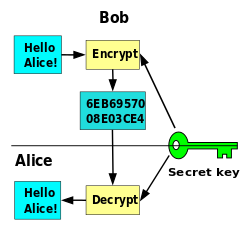
\includegraphics[width=55mm]{Symmetric_key_encryption.png}
  \centering
  \caption{Symmetric-key cryptography.}
  \label{fig:boat1}
\end{figure}
\noindent
\textbf{2. Decryption - Encryption in the middle}
\\In this system instead of having just two parties like above, one common third party(mostly a server) is added. So now, the sender and the server share a key(say K\textsubscript{a}), and the server and the receiver share a key(say K\textsubscript{b}). The sender's message is encrypted using K\textsubscript{a}, is decrypted at the server, then it is encrypted by K\textsubscript{b}, and sent to the receiver, where it finally gets decrypted and the message is delivered.
\end{document}


